\documentclass{article}
\usepackage[bottom=0.5cm, right=1.5cm, left=1.5cm, top=1.5cm]{geometry}
\usepackage{amsmath}
\usepackage{amssymb}
\usepackage{amsthm}
\usepackage{enumitem}
\usepackage{exercise} % Exercises Style
\usepackage{graphicx}
\usepackage{caption}
\usepackage{environ}
\newenvironment{solution}
  {\renewcommand\qedsymbol{$\blacksquare$}\begin{proof}[Solution]$ $}
  {\end{proof}}



% Enable Code
\usepackage{minted}
\let \extra T

\newcommand{\vect}[1]{\boldsymbol{#1}}
\newcommand{\E}{\mathbf{E}}
\DeclareMathOperator{\Tr}{Tr}
\DeclareMathOperator{\Cov}{Cov}
\DeclareMathOperator{\Var}{Var}
\DeclareMathOperator{\MSE}{MSE}


\title{Solutions to Assignment 2}
\author{Rongfei Jin}
\begin{document}
\maketitle

\section*{Conceptual 1}
\begin{enumerate}[label=(\alph*)]
  \item
        Flexible methods are better because there are enough samples to reduce variance without overfitting. Additionally, having a small number of predictors reduces the complexity of the flexible model—both in terms of search space and time complexity—compared to the same flexible model with more predictors. As a result, the flexible model can capture more information from the sample than inflexible methods.

  \item
        An inflexible method is preferable here. The small number of observations increases the variance of the model, making it more prone to overfitting. By contrast, an inflexible model makes fewer assumptions and is therefore less likely to overfit.

  \item
        A flexible method works better. Due to the strong linearity, an inflexible model cannot further reduce the bias, even if the dataset is large.

  \item
        An inflexible method is better in this situation. The high variance of the error terms suggests the sample might be somewhat incorrectly collected. A flexible model would try to fit the randomness introduced by the error terms, leading to a higher chance of overfitting.

\end{enumerate}
\section*{Conceptual 2}
\begin{enumerate}[label=(\alph*)]

  \item Regression: Salary is continuous. Inference is the focus here, since we want to understand what causes salary growth and utilize that information about the predictors.

  \item Classification: Success and failure are discrete outcomes. Inference is the focus here as well, since the company needs to identify the factors that lead to more success.

  \item Regression: The rate of change is continuous. We focus on prediction in this case, because we cannot alter any of the predictors but can still utilize insights about the rate of change.
\end{enumerate}

\newpage
\section*{Conceptual 5}

Advantages of Flexible method:
\begin{enumerate}
  \item is better at capturing the non-linearity
  \item  Allows greater modification based on specific area knowledge
  \item  Allows the change of pattern in data
\end{enumerate}
Disadvantages of Flexible method:
\begin{enumerate}
  \item  Has a higher chance of overfitting
  \item  has less interpretability
  \item  Requires more data
  \item  May have high time complexity
\end{enumerate}
Senarios where flexible methods are preferable

\begin{enumerate}
  \item The pattern is highly non-linear
  \item Our proposed model is very different from the assumptions of inflexible models
  \item The pattern evolutes over time
  \item We don't care about interpretability
\end{enumerate}
Senarios where inflexible methods are preferable
\begin{enumerate}
  \item The pattern is highly linear
  \item We want to interpret the model
  \item We have limited data
\end{enumerate}

\section*{Conceptual 6}

Parametric models assume functional forms of the models where the Non-Parametric models don't. Examples of parametric models linear, logistic regression, Linear SVM, Naive Bayes

\noindent
Advantages of Parametric models:

\begin{enumerate}
  \item has more interpretability
  \item works better on small datasets
  \item less likely to overfit
  \item requires less computations
\end{enumerate}
Disadvantages of Parametric method:
\begin{enumerate}
  \item may underfit the data when the true model is highly non-linear
  \item requires correct prior knowledge on the data to construct the model
\end{enumerate}

\section*{Conceptual 7}
we compute the euclidean distance by
\[
  d_i = \sqrt{X_{i1}^2 + X_{i2}^2 + X_{i3}^2}~\text{where } X_{ij} \text{ means the value jth predictor of ith observation }
\]

We can easily compute the values to be
\[\{d_1, d_2, d_3, d_4, d_5, d_6\} = \{3,2,3.16,2.24,1.41,1.73\}\]

when \(k=1\) we choose the one nearest neighbor which in this case is \(X_5\) thus the prediction is the same as the \(Y_5 = \text{Green}\)

when \(k=3\), we choose 3 nearest neighbor which is \(X_2, X_5, X_6\) and by majority vote the result is Red

if the decision boundry is highly non-linear, then we prefit a small \(k\) since a larger \(k\) will underfits the data by including votes that are not in the same group



\newpage
\section*{Applied 8}
\ifx \extra T
  \begin{minted}{r}
  # (a)
  college <- read.csv("College.csv")
  
  
  # (b)
  rownames(college) <- college[,1]
  college <- college[,-1]
  
  # (c) i
  summary(college)
  
  # (c) ii
  college[,1] <- as.factor(college[,1])
  pairs(college[,1:10])
  
  # (c) iii
  plot(college$Private, college$Outstate,
       main = "Boxplot of Outstate by Private",
       xlab = "Private",
       ylab = "Outstate",
       col  = "lightblue")
  
  # (c) iv
  Elite <- rep("No", nrow(college))
  Elite[college$Top10perc > 50] <- "Yes"
  Elite <- as.factor(Elite)
  college <- data.frame(college , Elite)
  
  plot(college$Elite, college$Outstate,
       main = "Boxplot of Outstate by Elite",
       xlab = "Elite",
       ylab = "Outstate",
       col  = "lightblue")
  
  par(mfrow = c(2, 2))
  hist(college$Top10perc, breaks = 5)
  hist(college$Top10perc, breaks = 10)
  hist(college$Top10perc, breaks = 15)
  hist(college$Top10perc, breaks = 20)
  # Elite schools have more top students but they cost more
  # Most non-elite schools only receive 20% of the top 10% from the high school class
  
  par(mfrow = c(1, 1))
  plot(college$Elite, college$S.F.Ratio,
       main = "Boxplot of S.F ratio by Elite",
       xlab = "Elite",
       ylab = "S.F. Ratio",
       col  = "lightblue")
  
  # An elite school may not have a higher S.F. Ratio than a non-elite school
  # And the overall difference in S.F Ratio is not large
\end{minted}
\fi

\if \extra T
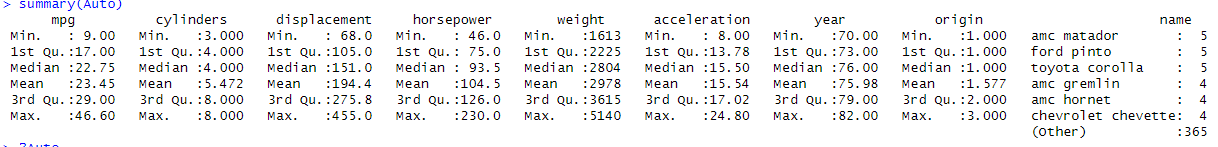
\includegraphics[scale=0.5]{s2.png}

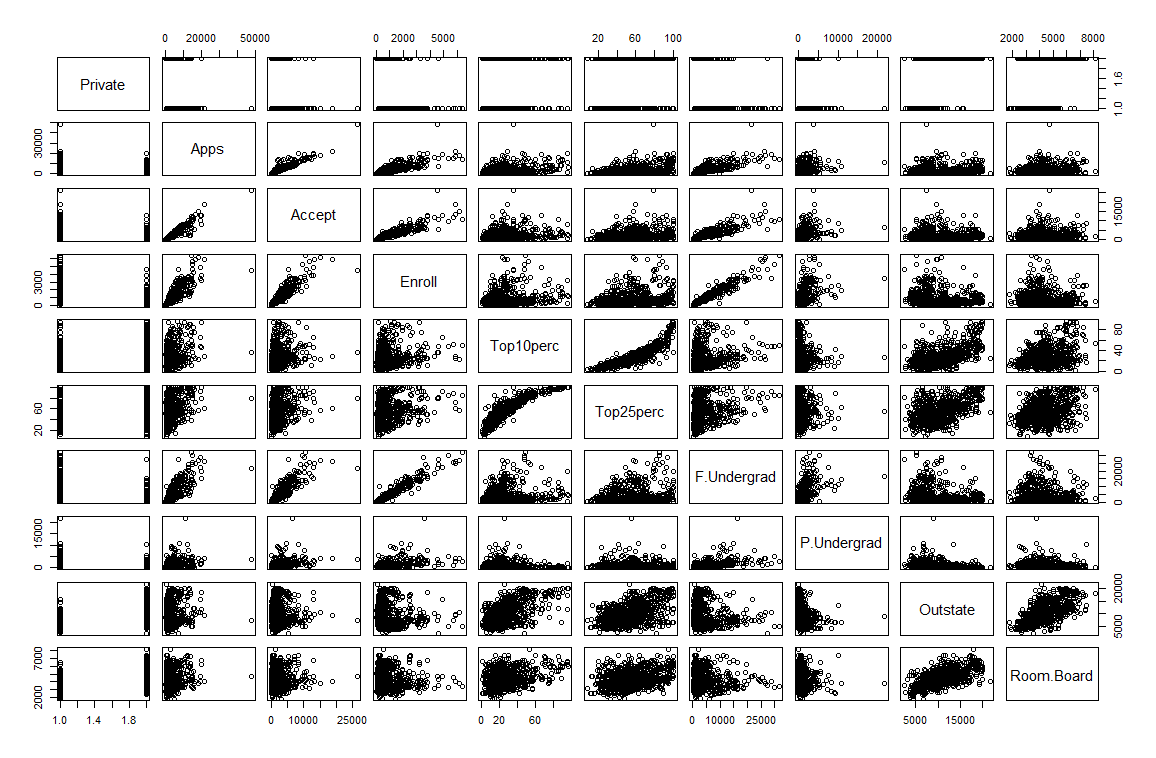
\includegraphics[scale=0.5]{cii.png}

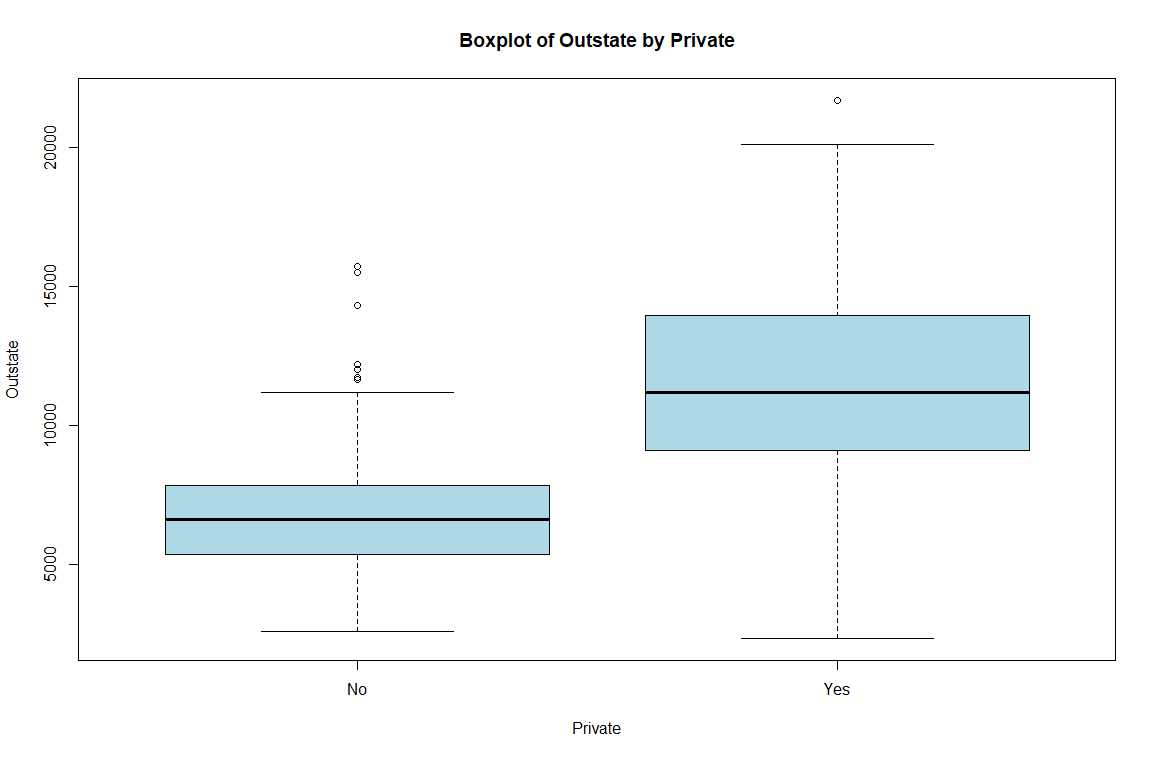
\includegraphics[scale=0.5]{ciii.png}

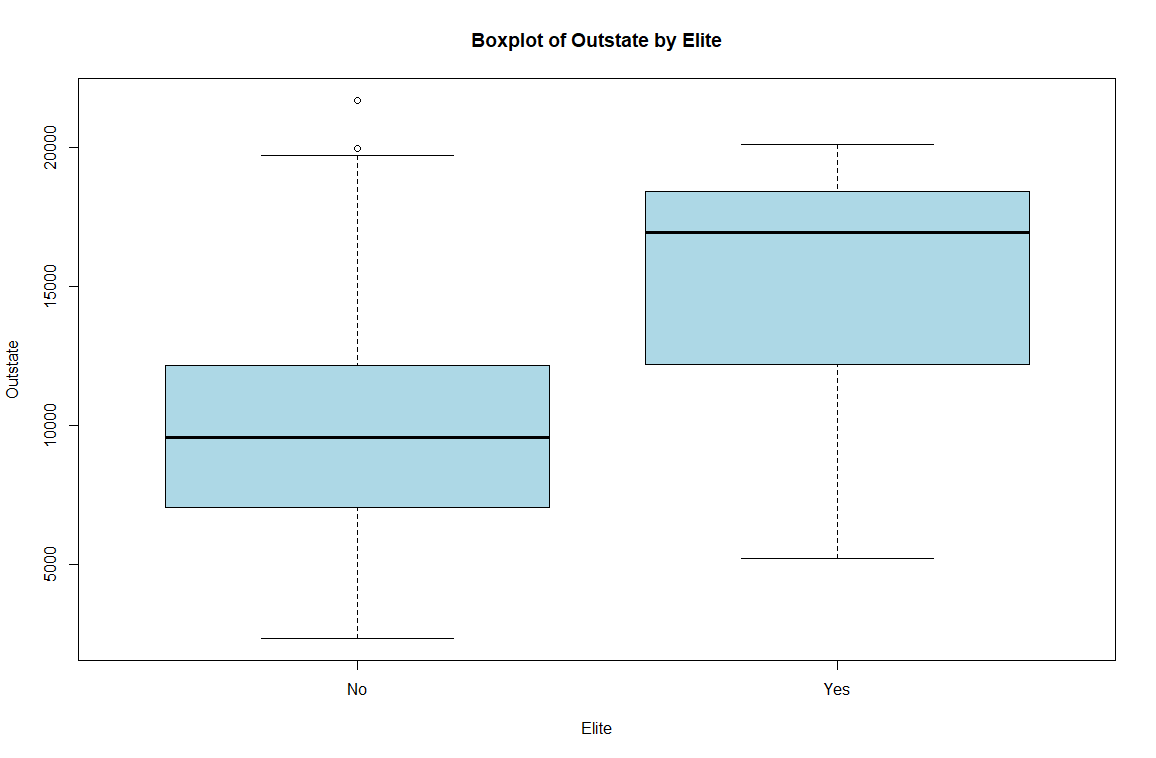
\includegraphics[scale=0.5]{civ.png}

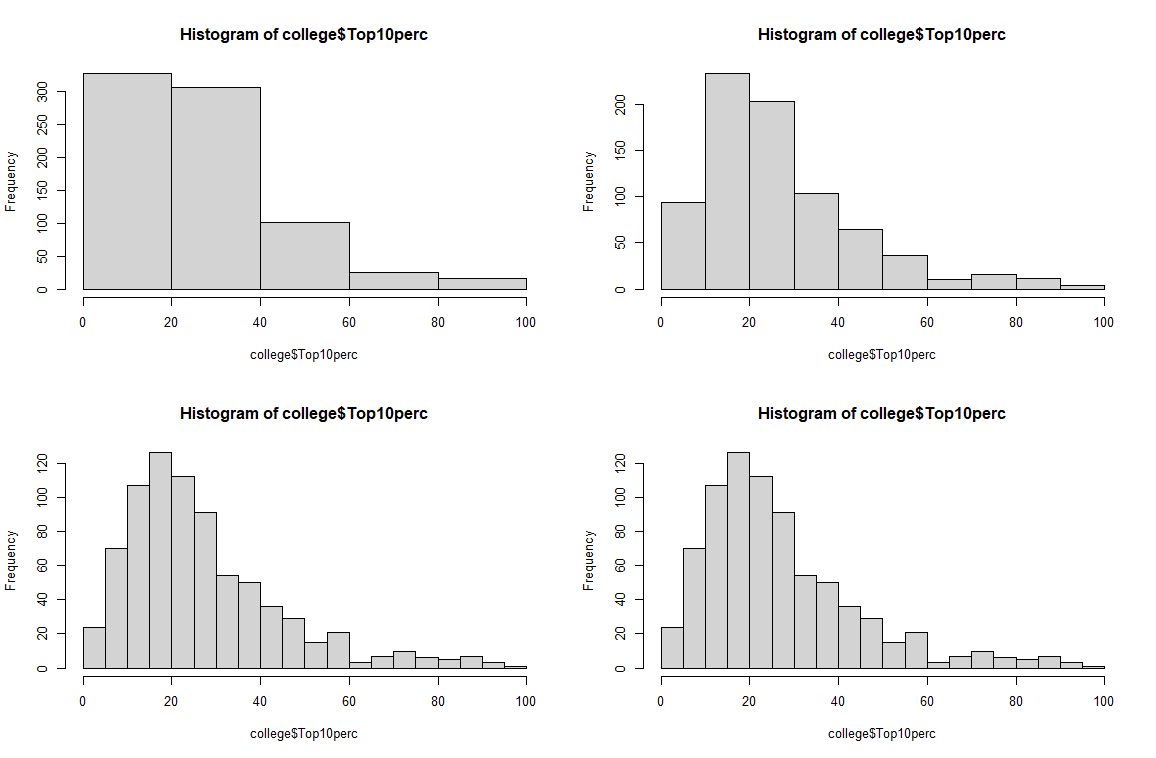
\includegraphics[scale=0.5]{cv.png}

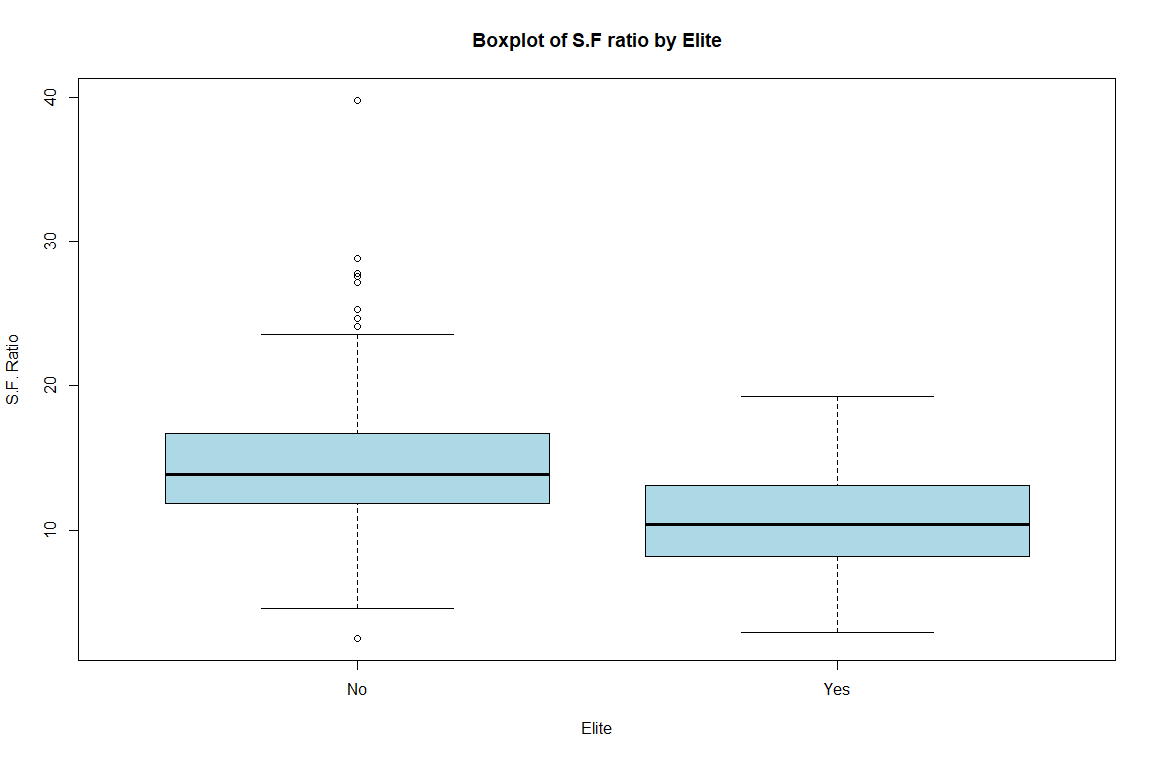
\includegraphics[scale=0.5]{cvi.png}
\fi


\newpage
\section*{Applied 9}

\ifx \extra T
\begin{minted}{r}
  library(ISLR2)

  # (a)
  summary(Auto)
  sapply(Auto, class)
  # Quantitative: mpg, displacement, horsepower, weight, acceleration, year
  # Qualitative: cylinders, origin
  
  # (b) (c)
  continuous = c("mpg", "displacement", "horsepower", "weight", "acceleration", "year")
  for (v in continuous) {
    cat(v,"\n")
    cat("range:", range(Auto[[v]]), "\t")
    cat("mean:", mean(Auto[[v]]), "\t")
    cat("sd:", sd(Auto[[v]]), "\n\n")
  }
  
  # (d)
  Auto_subset <- Auto[-c(10:85),]
  
  for (v in continuous) {
    cat(v,"\n")
    cat("range:", range(Auto_subset[[v]]), "\t")
    cat("mean:", mean(Auto_subset[[v]]), "\t")
    cat("sd:", sd(Auto_subset[[v]]), "\n\n")
  }
  
  pairs(Auto[,-ncol(Auto)])
  # More Cylinder means less mpg
  # Engine displacement and mpg are negatively related
  # Acceleration and mpg are not strongly correlated
  
  # (e)
  
  # A few variables can be used to predict mpg, 
  # such as cylinders, displacement, horsepower, weight 
  # because they shows strong linear pattern with mpg

\end{minted}
\fi

\ifx \extra T
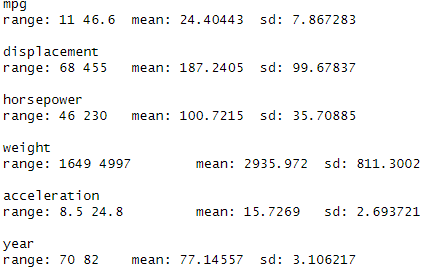
\includegraphics[scale=0.5]{s1.png}

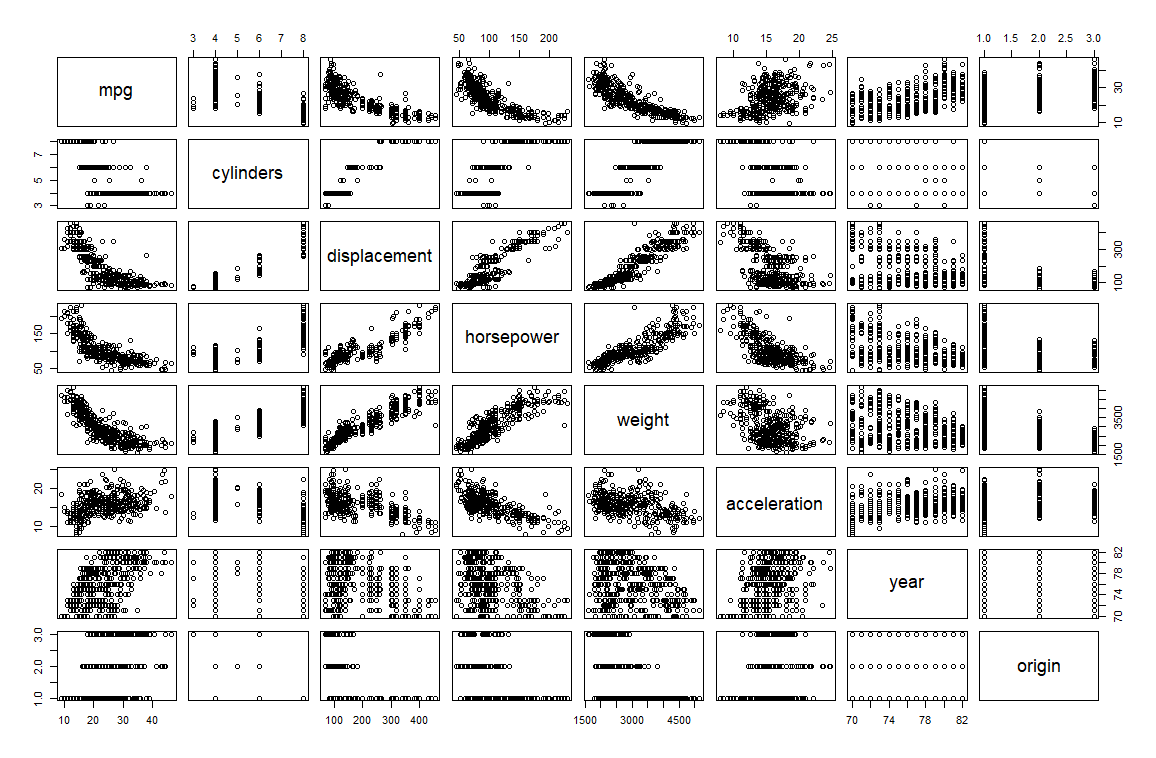
\includegraphics[scale=0.5]{e.png}
\fi

\newpage
\section*{Additional}
\begin{enumerate}[label=(\alph*)]

  \item
        For any points \((y_i, x_i)\), the residual can be expressed as \(\epsilon_i = y_i - \beta x_i\). The total residual sum of square is
        \[\text{RSS} = \sum_{i=1}^{n} (y_i - \beta x_i)^2 = \sum_{i=1}^{n} (y_i^2 - 2\beta x_i + \beta^2 x_i^2)\]

        We then minimize the RSS with respect to \(\beta\) by taking derivative of RSS
        \[
          \frac{d}{d\beta}(\text{RSS}) =  -2\beta\sum_{i=1}^{n} (y_ix_i) + 2\beta \sum_{i=1}^{n} x_i^2
        \]

        We set the derivative to 0 and obtain the solution to minimization

        \begin{align*}
          \frac{d}{d\beta}(\text{RSS}) & = 0 \\
        \end{align*}
        \begin{align*}
          \hat \beta & = \frac{\sum_{i=1}^{n} y_i x_i}{\sum_{i=1}^{n} x_i^2}
        \end{align*}

  \item

        We first check if the \(\hat \beta\) is not biased given \(\epsilon \sim N(0, \sigma^2)\)
        \begin{align*}
          \E(\hat \beta) & = \E(\frac{\sum_{i=1}^{n} (\beta x_i + \epsilon) x_i}{\sum_{i=1}^{n} x_i^2})                 \\
                         & = \frac{\E[\sum_{i=1}^{n} (\beta x_i^2 + x_i\epsilon)]}{\sum_{i=1}^{n} x_i^2}                \\
                         & = \frac{[\beta \sum_{i=1}^{n} x_i^2 + \E(\epsilon)\sum_{i=1}^{n} x_i]}{\sum_{i=1}^{n} x_i^2} \\
                         & = \frac{[\beta \sum_{i=1}^{n} x_i^2 + 0\cdot\sum_{i=1}^{n} x_i]}{\sum_{i=1}^{n} x_i^2}       \\
                         & = \beta
        \end{align*}

        \(\hat \beta\) is indeed unbiased, thus

        \begin{align*}
          \MSE(\hat \beta) & =  \Var(\hat \beta) + 0                                                        \\
                           & = \Var(\frac{\sum_{i=1}^{n} (\beta x_i + \epsilon) x_i}{\sum_{i=1}^{n} x_i^2}) \\
                           & = \frac{1}{(\sum_{i=1}^{n} x_i^2)^2} \Var(\epsilon) \sum_{i=1}^{n} x_i^2       \\
                           & = \frac{\sigma^2}{\sum_{i=1}^{n}x_i^2}
        \end{align*}

  \item
        For \(\beta\) to be unbiased, the residuals must be centered on 0, which means there's no intercept in the true model that causes a systemtatic shift to residuals, x and y must have a relationship that passes through the origin.

  \item
        \begin{align*}
          \hat \beta_1 - \hat \beta & = \frac{\sum_{i=1}^{n} (y_i - \bar y)(x_i - \bar x)}{\sum_{i=1}^{n} (x_i - \bar x)^2} - \frac{\sum_{i=1}^{n} y_i x_i}{\sum_{i=1}^{n} x_i^2}                                                                  \\
          \hat \beta_1 - \hat \beta & = \frac{\sum_{i=1}^{n} (y_ix_i - y_i \bar x - x_i \bar y + \bar y\bar x)}{\sum_{i=1}^{n} x_i^2 - 2x_i\bar x + \bar x^2} - \frac{\sum_{i=1}^{n} y_i x_i}{\sum_{i=1}^{n} x_i^2}                                \\
          \hat \beta_1 - \hat \beta & = \frac{(\sum_{i=1}^{n} y_ix_i) - n\bar y\bar x}{(\sum_{i=1}^{n} x_i^2) - n\bar x^2} - \frac{\sum_{i=1}^{n} y_i x_i}{\sum_{i=1}^{n} x_i^2}                                    & \sum_{i=1}^{n} x_i = n\bar x \\
        \end{align*}

        \(\hat \beta_1\) and \(\hat \beta\) are only the same if all \(x_i\) are centered on 0. If only centering \(y_i\), the bias persists.




\end{enumerate}

\end{document}


